\chapter{Requirements and specification engineering}

\section{Engineering principles}

A task contract translates stakeholder intent into a bounded change request. Functional requirements describe behavior; nonfunctional requirements describe security, performance, reliability and maintainability constraints. Invariants define properties that must remain true. Acceptance criteria should be observable and testable, with explicit non-goals and ownership.

\section{Implementation approach}

For a feature that adds a discount calculator, require integer cents, a bounded percentage, no floating-point rounding drift and unchanged public interfaces. Specify examples at zero, maximum and invalid input. Link each requirement to a test ID and define permitted paths. Capture base commit, max attempts, verification commands and approval requirements in a machine-readable task file. Validate the contract before dispatch.

\section{Verification and limitations}

A task is complete only when requirements are covered by trusted checks, the diff stays within scope and the owner accepts residual risk. Reject vague tasks such as improve security without a measurable outcome.

Figure~\ref{fig:d17} illustrates the conceptual flow from Requirements to Verification / release. The edges describe the proposed integration or control relationship, not undocumented internal calls.

\begin{figure}[htbp]\centering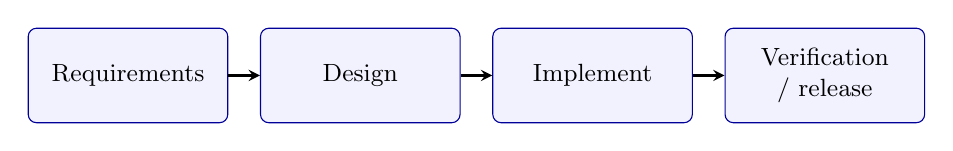
\begin{tikzpicture}[nodebox/.style={draw=blue!60!black,fill=blue!5,rounded corners=3pt,minimum height=12mm,text width=23mm,align=center,font=\small},>=stealth]
\node[nodebox] (n0) at (0.00,0.00) {Requirements};
\node[nodebox] (n1) at (2.95,0.00) {Design};
\node[nodebox] (n2) at (5.90,0.00) {Implement};
\node[nodebox] (n3) at (8.85,0.00) {Verification / release};
\draw[->,thick] (n0.east) -- (n1.west);
\draw[->,thick] (n1.east) -- (n2.west);
\draw[->,thick] (n2.east) -- (n3.west);
\end{tikzpicture}
\caption{Agentic SDLC (conceptual view).}\label{fig:d17}\end{figure}

\section{Chapter conclusion}

Apply the stated verification criteria before expanding the scope of this workflow. Record deviations, evidence and unresolved risks in the task record.
